\documentclass{sem6}

\institutename{Indian Institute of Information Technology, Vadodara}
\author{Dilip Puri}
\idt{201351014}
%\team{teamname}
%\collab{First Collaborator, Second Collaborator}

\coursename{Intro to AI}
\ccode{\begin{small}CS308\end{small}}
\profname{Mr. Parth Gupta}

\type{Assign}
\typeid{02}
\deadline{}%dd/mm/yyyy @hh:mm pm/am

\problemset{Perceptron, Pocket algo., Regression and Nonlinear Regression}

\begin{document}
\section{Implementing Perceptron}
In the Perceptron are going to classify data whether it is belongs to particular class or not so we have given dataset. Dataset consists features and their original belonging class.\\
For this problem we have given IRIS dataset there are three classes of in this dataset but we are going implement binary classification so either particular instance belongs to class or not?\\
Dataset have four features and class in name:
\begin{center}
\textbf{X = [petal$\_$length petal$\_$width sepal$\_$length sepal$\_$width class]\\}
\textbf{Classes: [Setosa Verginica Vermicolor]\\}
\end{center}
Now we are going to introduce \textbf{Weight vector} which will control the classification of instance of dataset.
\begin{center}
\textbf{w = [$w_1$ $w_2$ $w_3$ $w_4$]\\}
\end{center}
Our classification function will be like this:
\begin{center}
\textbf{Belongs to class if $\sum_{i=1}^d w_i*x_i > threshold$\\}
\textbf{Not belongs to class if $\sum_{i=1}^d w_i^T*x_i < threshold$\\}
\end{center}
so our formula be
\begin{center}
$H(x) = sign((\sum_{i=1}^d w_i*x_i)+b)$
\end{center}
\begin{flushright}
Where $x_1 \cdots x_4$ our features of vector x;\\
$H(x) = +1$ means ``belongs to class"\\
$H(x) = -1$ means ``not belongs to class"\\
Note :- Our class is \textbf{``Setosa"\\}
The weights are $w_1 \cdots w_d$, and the threshold is determined by the bias term b.
\end{flushright}
Now the learning of the Perceptron is Weight so the algorithm will determine what w should be. Our learning algorithm will find this w using a simple iterative method. And we have update rule for w is if we have $y(t) \neq sign(w(t)*x(t))\hspace*{2cm} w(t+1) = w(t) + y(t)*x(t)\\ $
\newpage
\textbf{Results and Graphs}
\lstinputlisting[language=Octave]{../perceptron/perceptron.txt}
\begin{center}
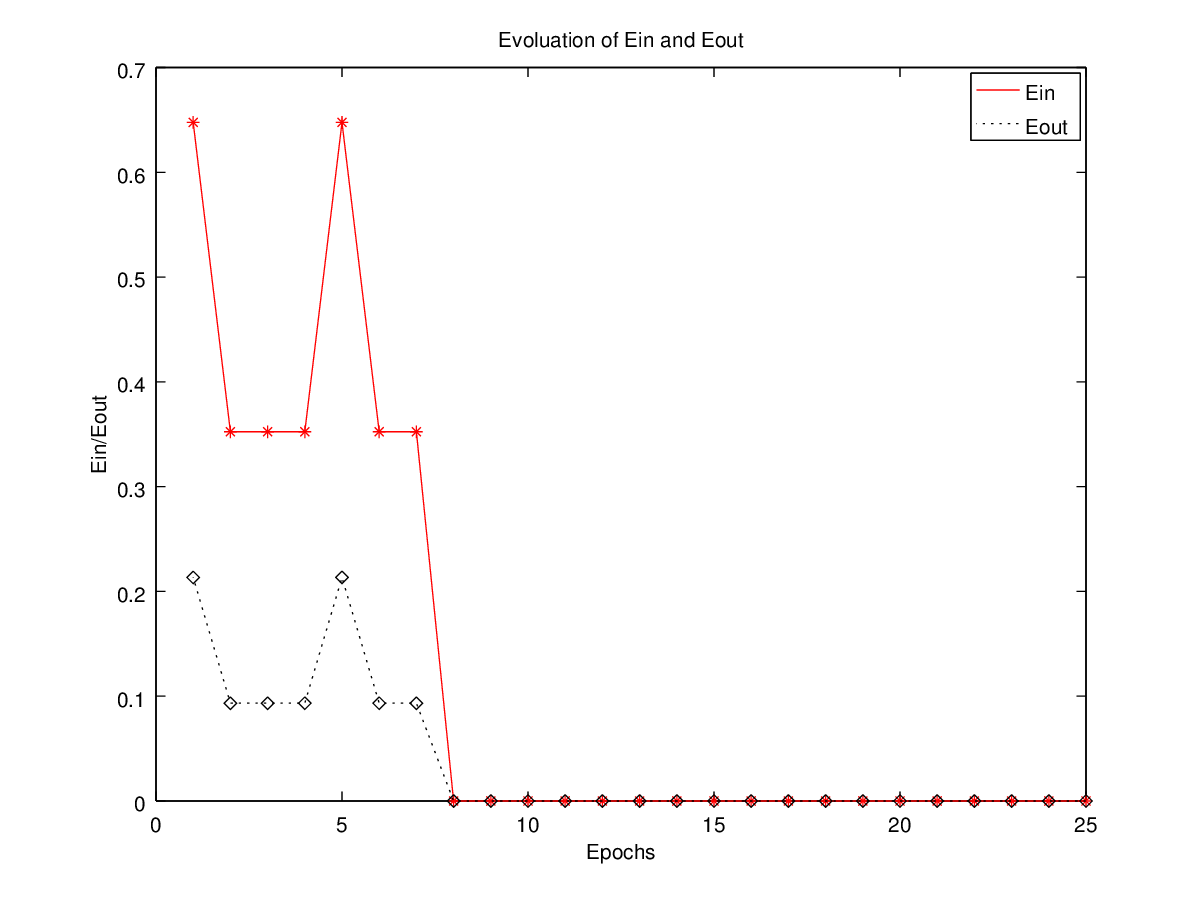
\includegraphics[scale=.6]{../perceptron/perceptron.png}
\end{center}
\lstinputlisting[language=Octave]{../perceptron/weight.txt}
\newpage
\begin{figure}[!tbp]
\centering
\begin{minipage}[b]{0.45\textwidth}
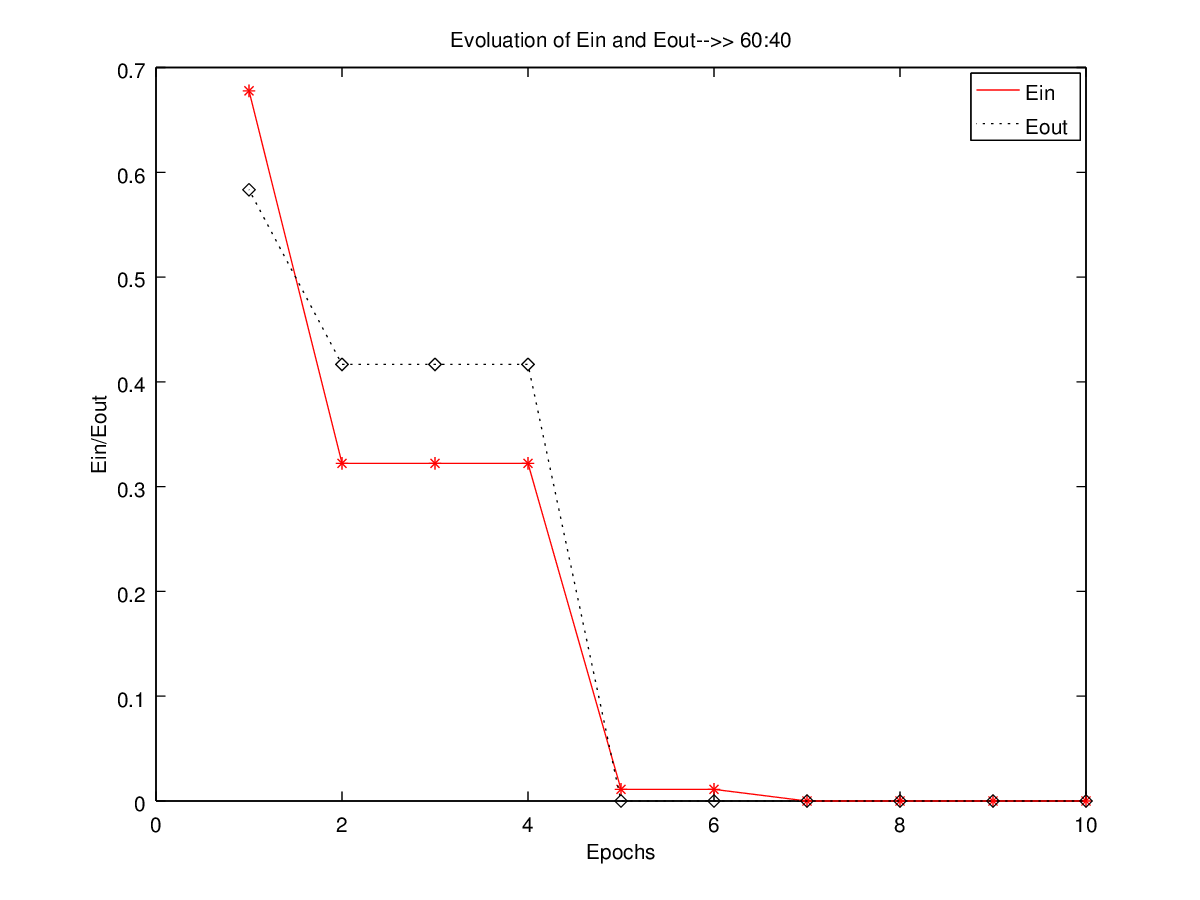
\includegraphics[width=\textwidth]{../perceptron/perceptron2.png}
\caption{Train:Test::60:40}
\end{minipage}
\hfill
\begin{minipage}[b]{0.45\textwidth}
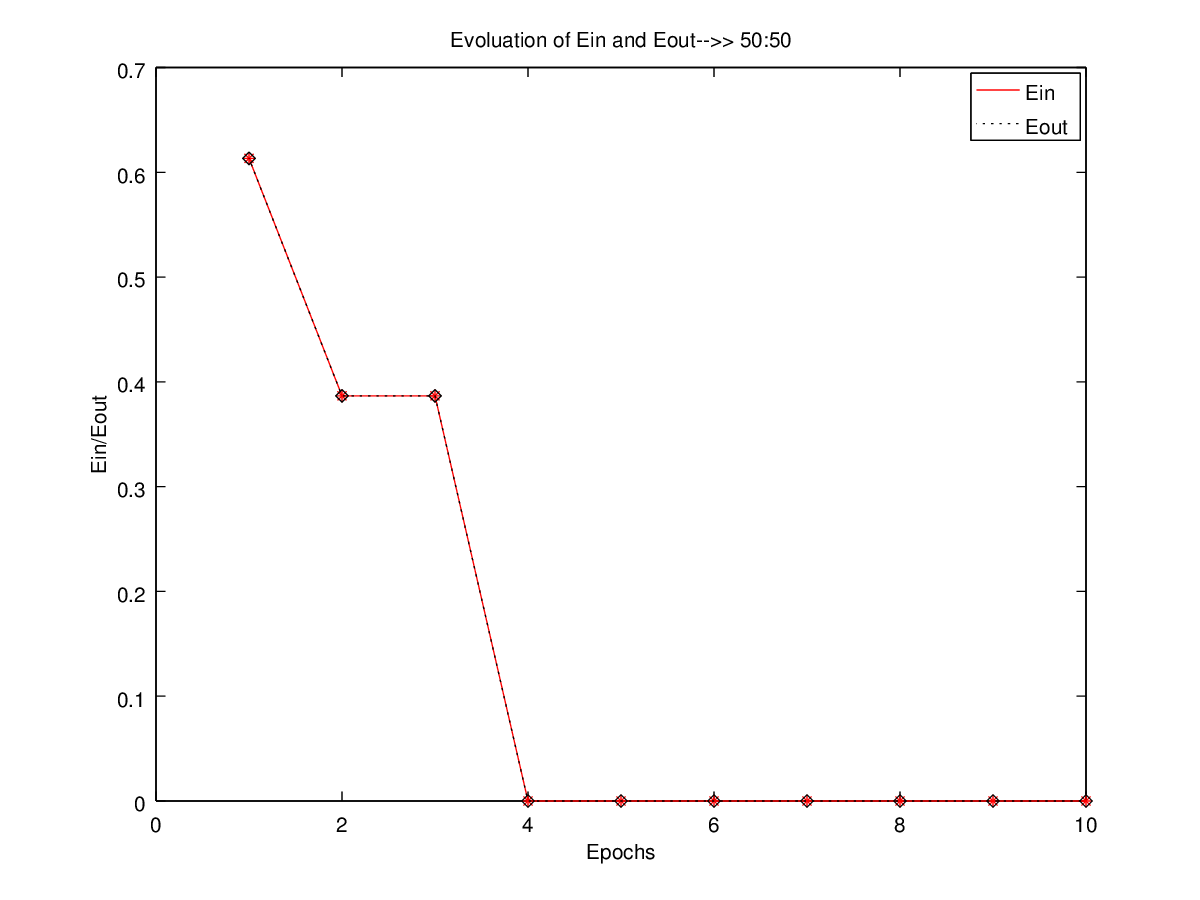
\includegraphics[width=\textwidth]{../perceptron/perceptron3.png}
\caption{Train:Test::50:50}
\end{minipage}
\end{figure}

\begin{figure}[!tbp]
\centering
\begin{minipage}[b]{0.45\textwidth}
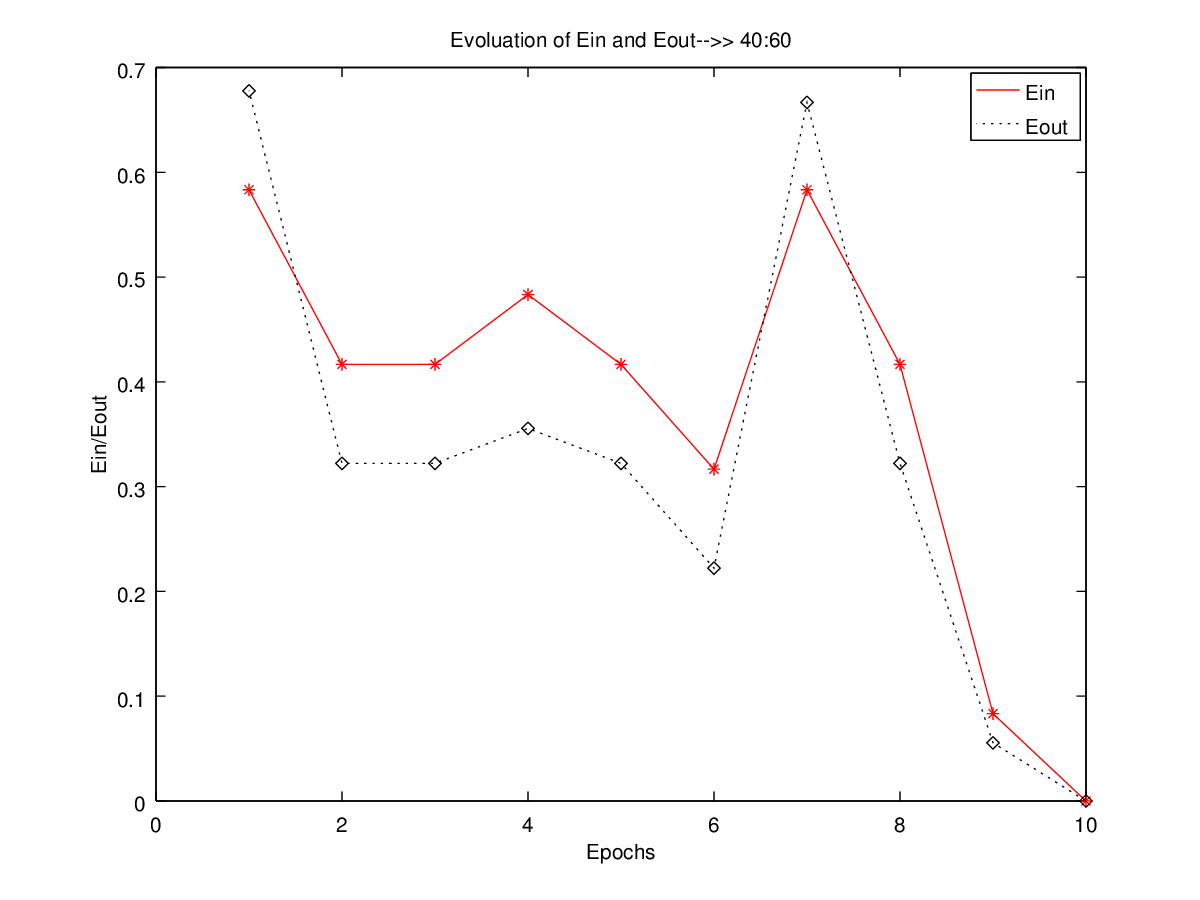
\includegraphics[width=\textwidth]{../perceptron/perceptron4.png}
\caption{Train:Test::40:60}
\end{minipage}
\hfill
\begin{minipage}[b]{0.45\textwidth}
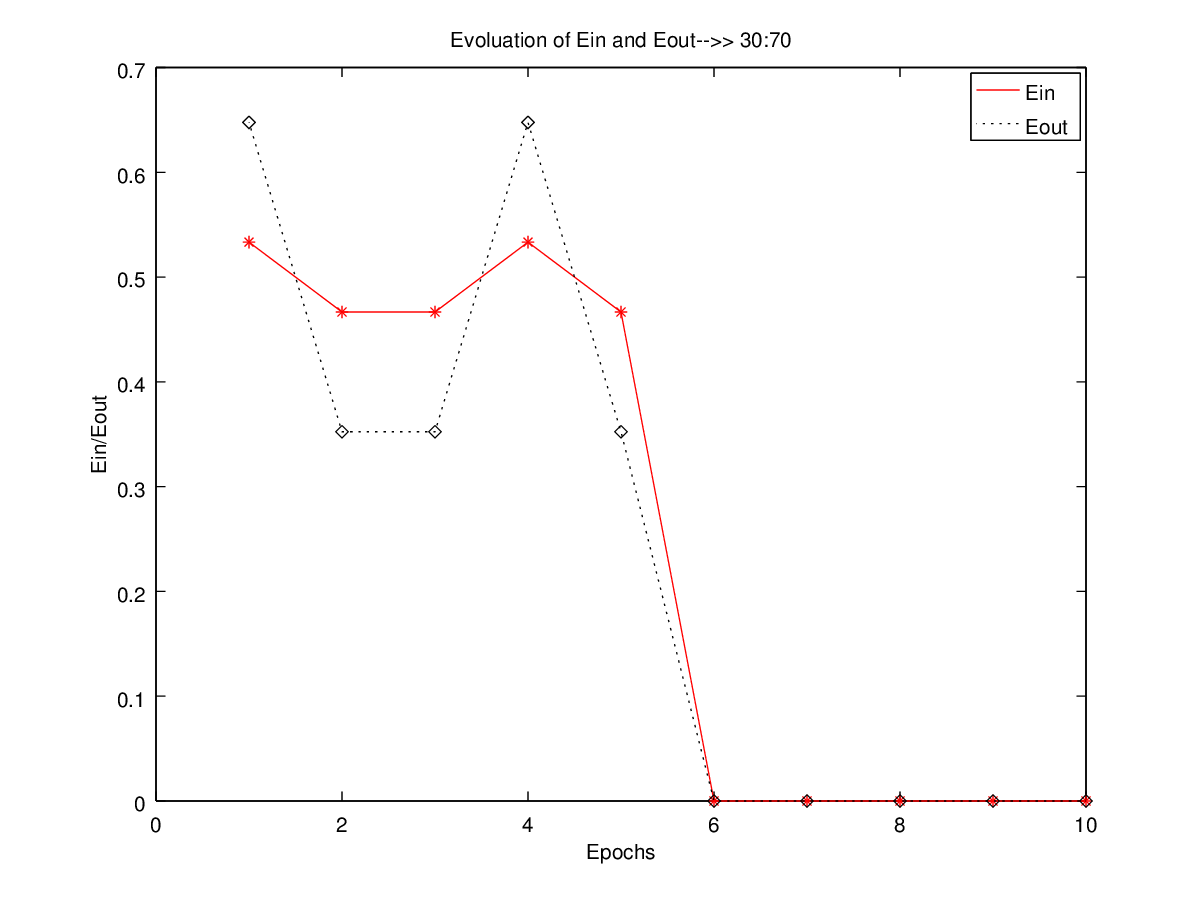
\includegraphics[width=\textwidth]{../perceptron/perceptron5.png}
\caption{Train:Test::30:70}
\end{minipage}
\end{figure}


\newpage
\section{Pocket Algorithm}
\begin{center}
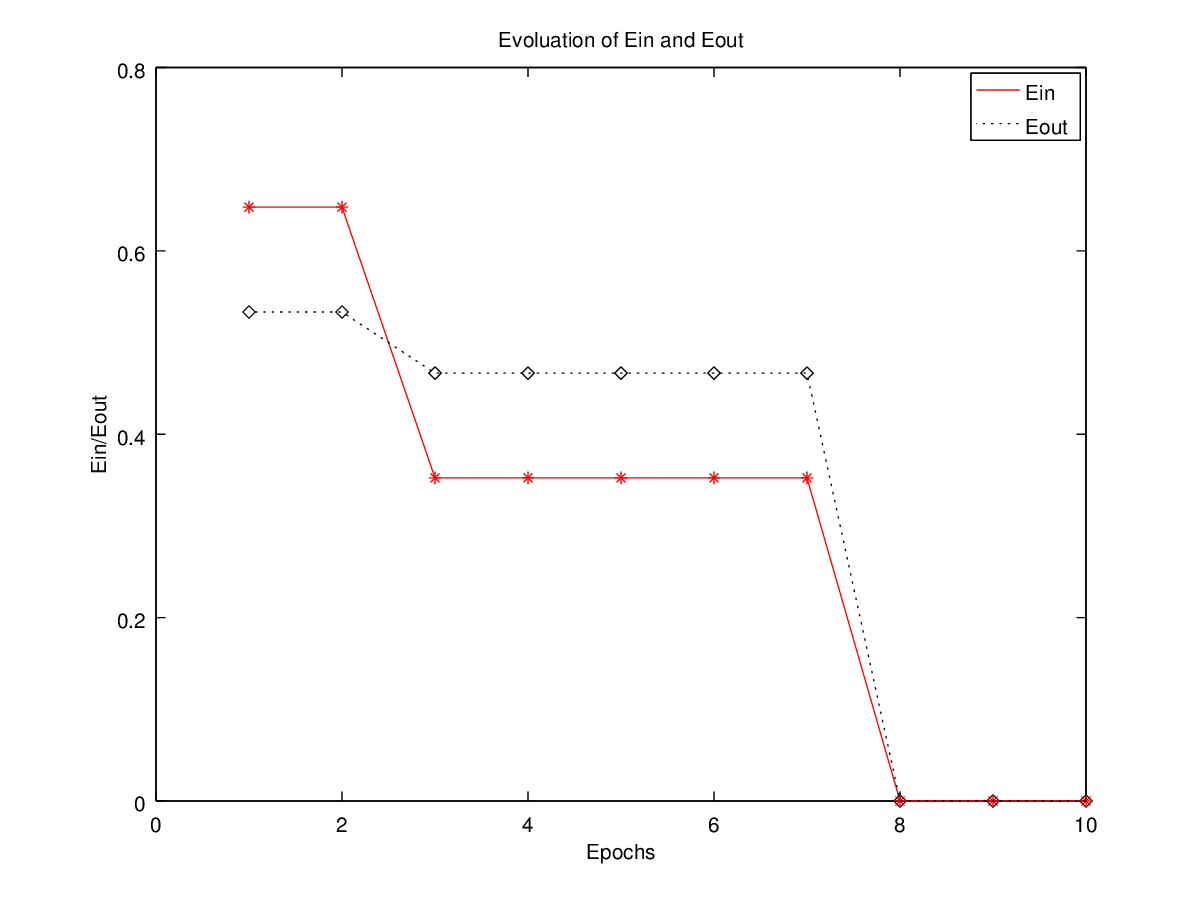
\includegraphics[scale=.6]{../perceptron/pocket.png}
\end{center}

\section{Regression and Nonlinear Regression}
\lstinputlisting[language=Octave]{../regression/weight.txt}

\end{document}